\documentclass[10pt,a4paper,openright]{article}
\usepackage{amsfonts}
\usepackage{float}
\usepackage[utf8]{inputenc}
\usepackage[T1]{fontenc}
\usepackage{graphicx}
\usepackage{amsmath,amssymb,verbatim}
\textheight=240mm
\textwidth=170mm
\topmargin=-15mm
\oddsidemargin=-6mm
\evensidemargin=\oddsidemargin
\newcommand\tab[1][1cm]{\hspace*{#1}}
\usepackage{hyperref}
\newcommand{\norm}[1]{\left\lVert#1\right\rVert}

\begin{document}
	\begin{flushleft}
		\large Name: Matouš Dzivjak\\
		\large Date: 9.11.2018\\
	\end{flushleft}
\begin{center}
	\huge PCA
\end{center}
\section{Zadání}
\begin{verbatim}
https://gitlab.fel.cvut.cz/B0B33OPT/public/blob/master/cviceni/03_pca/03_pca.pdf
\end{verbatim}


\section{Řešení 1. části}
\subsection{}
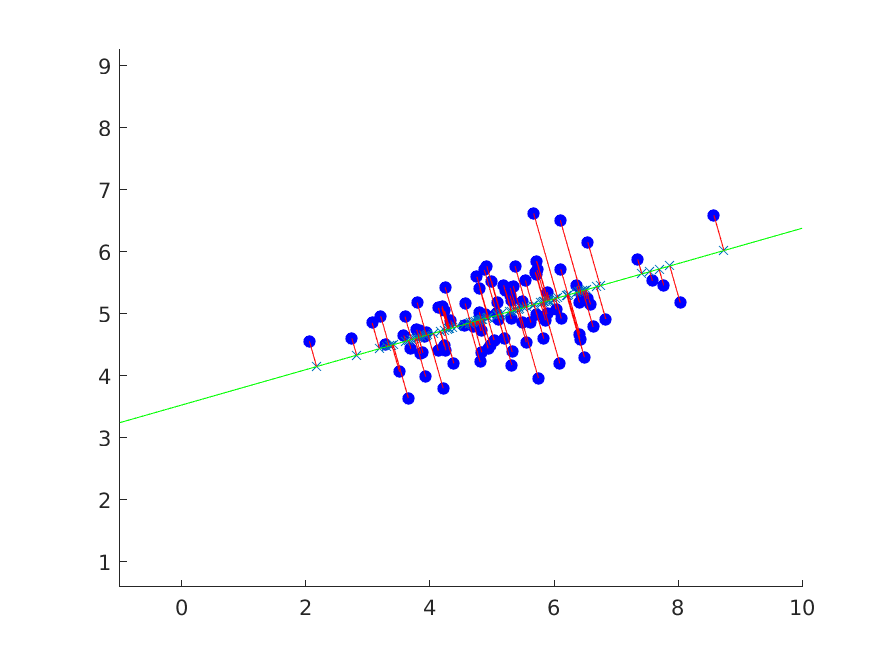
\includegraphics[scale=0.8]{line.png}

\subsection{}
\begin{center}
Součet čtverců kolmých vzdáleností je $err = 24.2419$
\end{center}

\subsection{}
\begin{center}
    Nejdříve máme řešení reprezentovat ve formě $\{ y \in \R ^ 2 | y ^ T \cdot x = \alpha \}$\\
    Kde
    \[y =
    \begin{bmatrix}
        y_1\\
        y_2
    \end{bmatrix}\]
    \[x =
    \begin{bmatrix}
        x_1\\
        x_2
    \end{bmatrix}\]
    Po roznásobení pro přímku dostáváme rovnici\\
    $y_1 \cdot x_1 + y_2 \cdot x_2 = \alpha$\\
    Po dosazení normálového vektoru přímky $n$ (kolmý na směrový vektor přímky, za $y_1$ a $y_2$)
    a souřadnice těžiště bodů (za $x_1$ a $x_2$)
    dostáváme $\alpha = -3.3931$\\
    \[y =
    \begin{bmatrix}
        -0.2740\\
        0.9617
    \end{bmatrix}\]
    \[x =
    \begin{bmatrix}
        5.1231\\
        4.9876
    \end{bmatrix}\]
    V druhé části máme řešení reprezentovat ve formě: $\{y_0 + t \cdot s | t \in \R \}$.
    To však máme stíženo a omezeno podmínkou, že norma $\norm{y_0}$ musí být minimální. Tedy
    musíme nalézt bod na přímce, který je nejblíže počátku (zatím co jinak bychom mohli použít například
    již nalezené těžiště bodů).
\end{center}

\section{Řešení 2. části}

\subsection{}
\begin{center}
Tabulka s optimálními hodnotami kritéria pro $r \in \{1,2,5,10,15\}$\\
\begin{tabular}{|r|l|}
    \hline
    r & $\sum_{i=1}^{m} \norm{\tilde{a_i} - a_i}^2$ \\
    \hline \hline
    1 & $4.6166 \cdot 10^8$ \\
    2 & $1.6925 \cdot 10^8$ \\
    5 & $1.0453 \cdot 10^7$\\
    10 & $1.1982 \cdot 10^6$\\
    15 & $2.5626 \cdot 10^5$\\
    \hline
\end{tabular}
\end{center}

\subsection{}
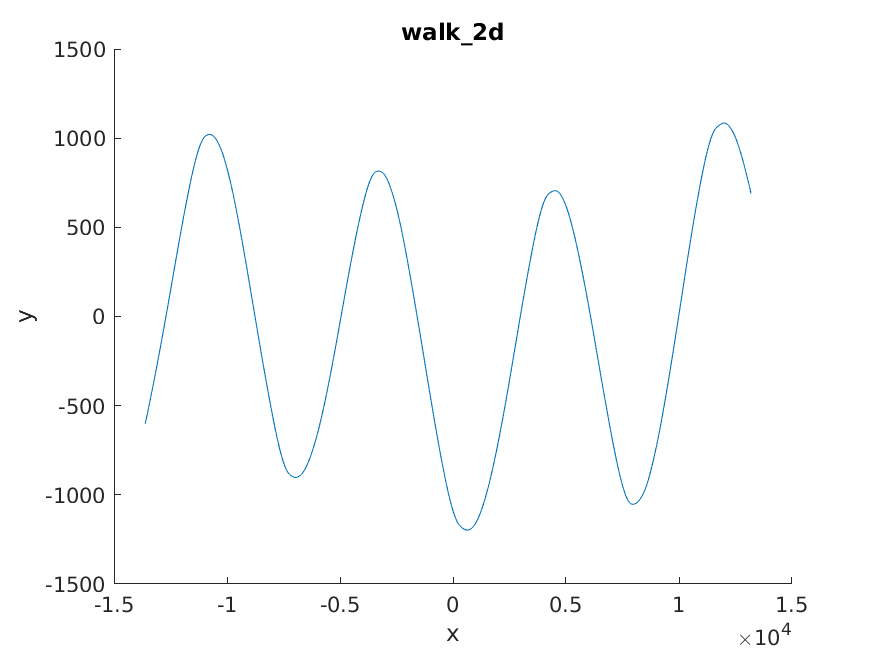
\includegraphics[scale=0.5]{walk_2d.png}
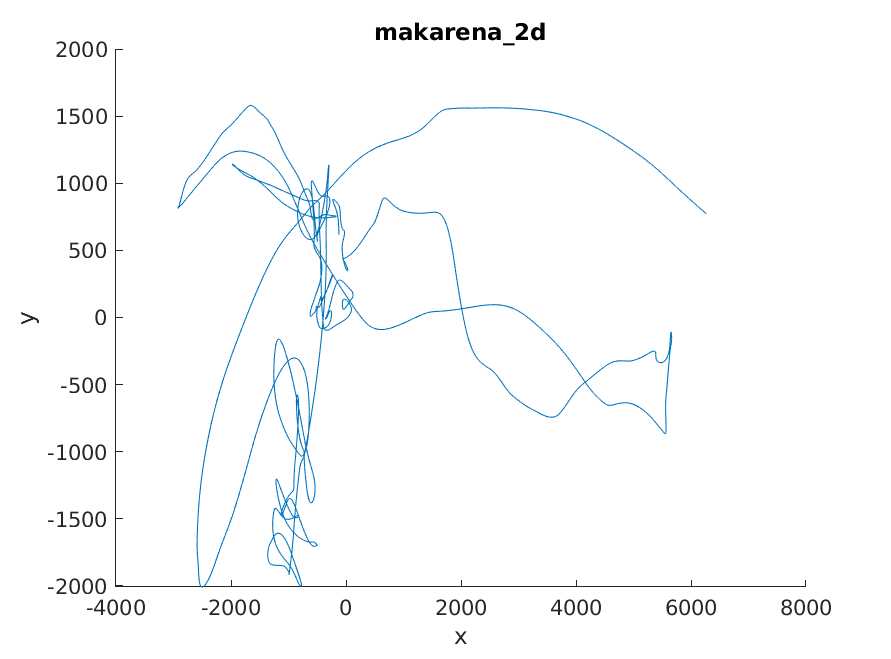
\includegraphics[scale=0.5]{makarena_2d.png}\\
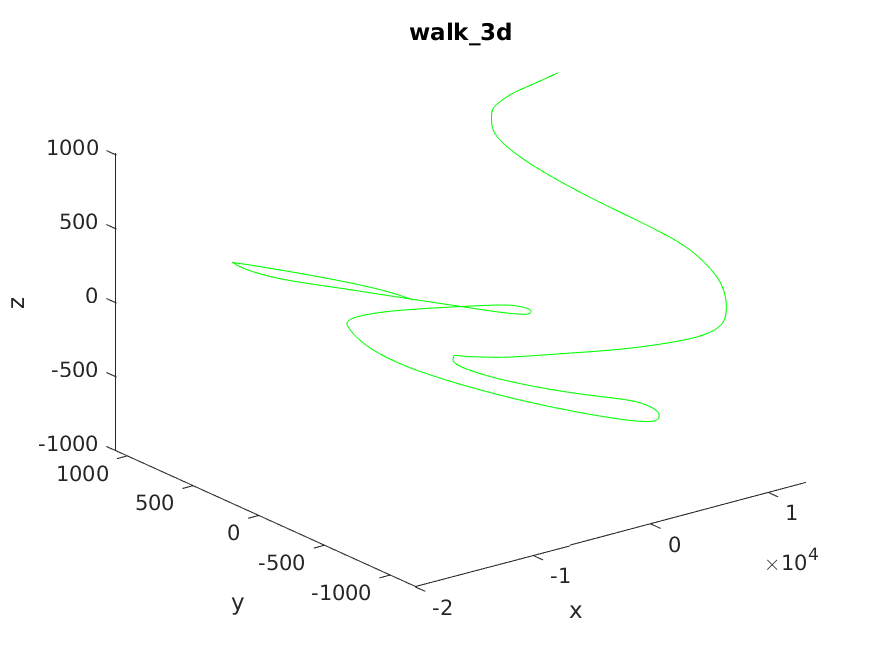
\includegraphics[scale=0.5]{walk_3d.png}
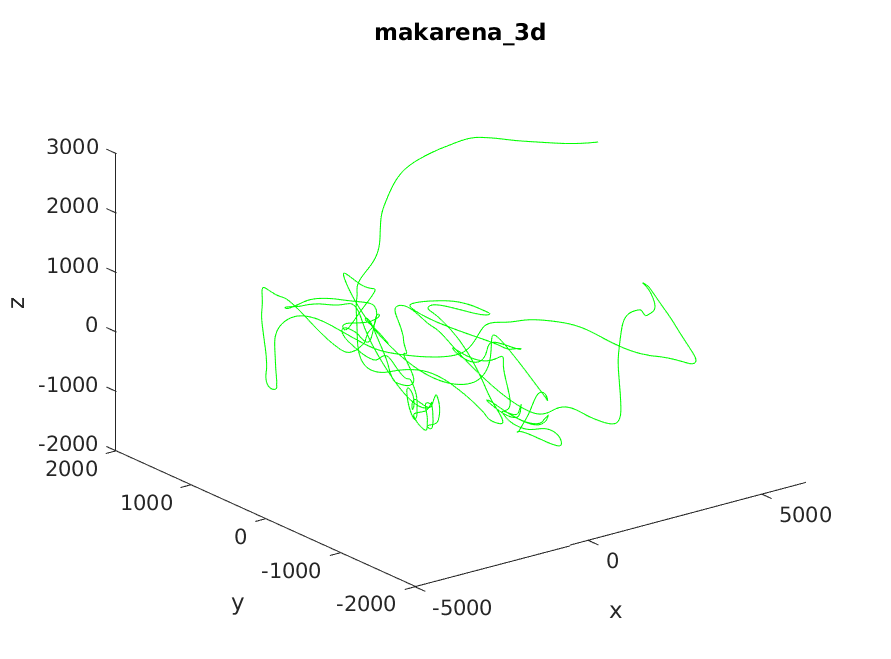
\includegraphics[scale=0.5]{makarena_3d.png}\\

\subsection{}
Pokud se body pohybují pouze po přímce stačí nám pro dosažení nulové aproximační chyby podprostor dimenze 1.
Tedy zredukujeme reprezentaci na vektor reálných čísel, která budou udávat offset na přímce, po které se body pohybují.

\subsection{}


\end{document}